% https://texnique.fr/osqa/questions/6660/tikz-alignement-de-nodes/6663
\documentclass{beamer}
\usepackage{tikz}
\begin{document}
\begin{frame}
    \frametitle{Occupation du site de Bibracte}
    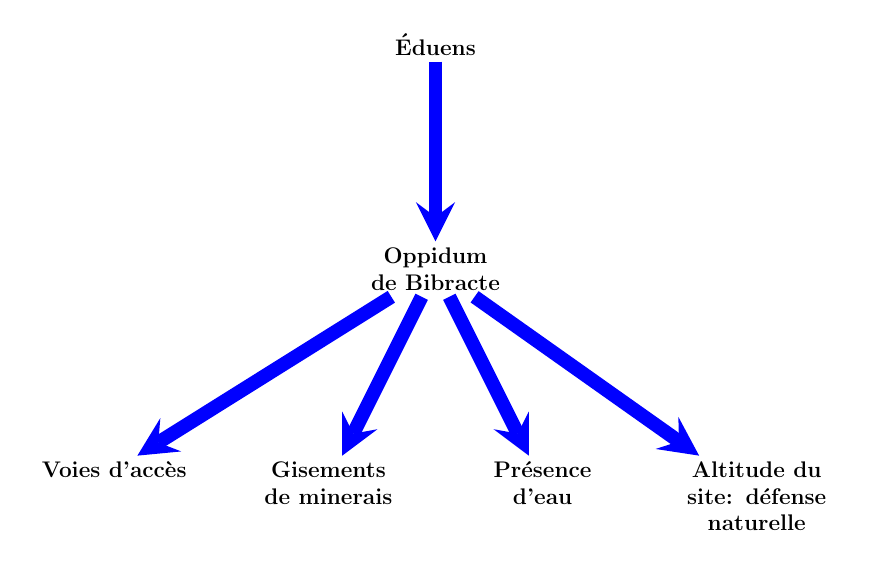
\begin{tikzpicture}[
        scale=.68,
        every node/.style={scale=.68},
        quadri/.style={rectangle,draw,fill=white},
        case/.style={text width=3cm,text centered,anchor=north,font=\large\bfseries},
        myarrow/.style={-stealth,line width=5pt,blue}
    ]
% Cases
    \node[case] (Ed) at (0,4) {Éduens};
    \node[case] (Opp) at (0,0) {Oppidum de Bibracte};
    \node[case] (Acc) at (-6,-4) {Voies d'accès};
    \node[case] (Gis) at (-2,-4) {Gisements de minerais};
    \node[case] (Eau) at (2,-4) {Présence d'eau};
    \node[case] (Def) at (6,-4) {Altitude du site: défense naturelle};

% Flèches
    \draw[myarrow] (Ed) to (Opp); 
    \draw[myarrow] (Opp) to (Acc);
    \draw[myarrow] (Opp) to (Gis);
    \draw[myarrow] (Opp) to (Eau);
    \draw[myarrow] (Opp) to (Def);
    \end{tikzpicture}
\end{frame}
\end{document}